\documentclass{article}
\usepackage{mathtools}
\usepackage{amsmath}
\usepackage{amssymb}
\usepackage{amsfonts}
\usepackage{graphicx}
\usepackage{float}

\linespread{1.3}
\setlength{\parindent}{0em}
\setlength{\parskip}{1em}
\setcounter{secnumdepth}{0}
\setcounter{MaxMatrixCols}{20}

\title{Assignment 1}
\author{Joshua Hwang (44302650)}
\date{27 March}

\begin{document}
\maketitle

\section{Problem Sheet 2 Question 1}
We must make sure the code is linear before creating a generator matrix.
It is a linear code if it's a subspace; closed under component wise addition
and scalar multiplication. Since we are in $GF[2]$ scalar multiplicataion is
either 0 or 1 which means scalar mutliplication is closed as $\vec{0}$ is
in the code. Consider $u = x_u y_u a_u z_u b_u$ and $v = x_v y_v a_v z_v b_v$.

\begin{align*}
    u + v
    &= \begin{bmatrix}
        x_u \\
        y_u \\
        a_u \\
        z_u \\
        b_u
    \end{bmatrix}
    +
    \begin{bmatrix}
        x_v \\
        y_v \\
        a_v \\
        z_v \\
        b_v
    \end{bmatrix} \\
    &= \begin{bmatrix}
        x_u + x_v \\
        y_u + y_v \\
        a_u + a_v \\
        z_u + z_v \\
        b_u + b_v
    \end{bmatrix}
    && \text{Use definitions of $a$ and $b$} \\
    &= \begin{bmatrix}
        x_u + x_v \\
        y_u + y_v \\
        x_u + y_u + x_v + y_v \\
        z_u + z_v \\
        y_u + z_u + y_v + z_v
    \end{bmatrix} \\
    &= \begin{bmatrix}
        (x_u + x_v) \\
        (y_u + y_v) \\
        (x_u + x_v) + (y_u + y_v) \\
        (z_u + z_v) \\
        (y_u + y_v) + (z_u + z_v)
    \end{bmatrix} \\
\end{align*}

This satifies the definition of the codes thus is a subspace and a linear code.

Through analysis we notice can use the definition of the encoding to find the
basis for the mapping. To make it clearer we will swap the order of the
final sequence, we will transform the code back at the end.
\begin{align*}
    xyz &\to xyzab \\
    100 &\to 10010 \\
    010 &\to 01011 \\
    001 &\to 00101 \\
\end{align*}

Our generating matrix is now,
\begin{align*}
    \begin{bmatrix}
        1 & 0 & 0 & 1 & 0 \\
        0 & 1 & 0 & 1 & 1 \\
        0 & 0 & 1 & 0 & 1
    \end{bmatrix}
\end{align*}

And our respective parity check matrix is,
\begin{align*}
    \begin{bmatrix}
        1 & 0 \\
        1 & 1 \\
        0 & 1 \\
        1 & 0 \\
        0 & 1
    \end{bmatrix}
\end{align*}

From here we must remember to swap the rows that were previously swapped
columns. Row 4 will be swapped to Row 3.
\begin{align*}
    \begin{bmatrix}
        1 & 0 \\
        1 & 1 \\
        1 & 0 \\
        0 & 1 \\
        0 & 1
    \end{bmatrix}
\end{align*}

Copying this process for the generator matrix will give us the true
generating matrix.
\begin{align*}
    \begin{bmatrix}
        1 & 0 & 0 & 1 & 0 \\
        0 & 1 & 0 & 1 & 1 \\
        0 & 0 & 1 & 0 & 1
    \end{bmatrix}
    &\to 
    \begin{bmatrix}
        1 & 0 & 1 & 0 & 0 \\
        0 & 1 & 1 & 0 & 1 \\
        0 & 0 & 0 & 1 & 1
    \end{bmatrix} \\
\end{align*}

\section{Problem Sheet 2 Question 6}
We first show certain attributes of Hamming weight.
Consider a code with weighting $n$ called $c_1$. Let's look at what happens
when we add it to another code, $c_2$.
Of those $n$ bits it adds $r$ bits to $c_2$.
The remaining $n-r$ bits will end up cancelling with bits in $c_2$.
Now,
\begin{align*}
    |c_1 + c_2| &= |c_2| + r - (n - r) \\
    &= |c_2| + 2r - n
\end{align*}

If $n$ is even the eveness of $|c_1 + c_2|$ is determined by $|c_2|$.
If $n$ is odd the even/odd weighting is opposite of $|c_2|$.

We now use induction by adding new codes, odd or even, to the
linear code's basis.

First, a base case. Since every linear code must have the word with all 0s
a code with two basis words is either half even or completely even.

Now assume we know this works for $k$ base code words
notated by $c_1$ to $c_k$. Let $|S|$ and $|S_{even}|$ be the number
of words and  even words respectively in the code (not just base),
this may also be the number of odd words if it isn't 0.
Now we add a new base word to the code, $c_{k+1}$.
Now each word is represented by
\begin{align*}
    w &= \alpha_1 c_1 + \alpha_2 c_2 + ... + \alpha_k c_k
    + \alpha_{k+1} c_{k+1}
\end{align*}

The code is now evenly split by those with $\alpha_{k+1} = 0$
and $\alpha_{k+1} = 1$ since $|S|$ could be seen as all words with
$\alpha_{k+1} = 0$. Our new code will have $2\times|S|$.
If the new word, $c_{k+1}$, is even then we have $2\times|S_{even}|$ even
words, the even words with $\alpha_{k+1} = 0$
and those with $\alpha_{k+1} = 1$.
Therefore we still maintain completely even or half even.

If the new word, $c_{k+1}$, is odd then we have $|S_{odd}| + |S_{even}|$ even
words, the even
words with $\alpha_{k+1} = 0$ and the previously odd words
with $\alpha_{k+1} = 1$. Using the same reasoning we have
$|S_{odd}| + |S_{even}|$ odd words. Therefore, the number of even and odd words
is equal.

We have now proven this for the $k+1$ case. Therefore, by induction, the
code will ever only have all even or half even weighted words.

\section{Problem Sheet 3 Question 4}
\subsection{Part a}
A Hamming code (15,11) has 4 parity bits at positions 1, 2, 4 and 8. We will
denote each position in the word by, $c_i$ for each position $i$. For the
original word we have $w_i$.
Each parity bits is determined by,
\begin{align*}
    c_1 &= w_1 + w_3 + w_5 + w_7 + w_9 + w_{11} \\
    c_2 &= w_2 + w_3 + w_6 + w_7 + w_{10} + w_{11} \\
    c_4 &= w_4 + w_5 + w_6 + w_7 \\
    c_8 &= w_8 + w_9 + w_{10} + w_{11}
\end{align*}

We know a Hamming code is linear since all the parity check bits are determined
by bitwise additions which are linear, (refer the Problem Sheet 2 Question 1).
Thus we CAN create a parity check matrix. To simplify the process we will
use column swaps and move all parity swap bits to the end of the word.

By using the standard basis of non-encoded words, ($00000000001$,
$00000000010$, ...) our basis for the encoded words comes out naturally to be
\begin{align*}
    \left[ I_{11\times11} | P_{11\times4} \right] \\
\end{align*}

Keep in mind the columns are swapped so the parity bits are all at the right
and the left hand side is the standard basis of the non-encoded words. We now
calculate the rows in $P$.
\begin{align*}
    \begin{bmatrix}
        1 & 0 & 0 & 0 \\
        0 & 1 & 0 & 0 \\
        1 & 1 & 0 & 0 \\
        0 & 0 & 1 & 0 \\
        1 & 0 & 1 & 0 \\
        0 & 1 & 1 & 0 \\
        1 & 1 & 1 & 0 \\
        0 & 0 & 0 & 1 \\
        1 & 0 & 0 & 1 \\
        0 & 1 & 0 & 1 \\
        1 & 1 & 0 & 1
    \end{bmatrix}
\end{align*}

We now create our parity check.
\begin{align*}
    \begin{bmatrix}
        1 & 0 & 0 & 0 \\
        0 & 1 & 0 & 0 \\
        1 & 1 & 0 & 0 \\
        0 & 0 & 1 & 0 \\
        1 & 0 & 1 & 0 \\
        0 & 1 & 1 & 0 \\
        1 & 1 & 1 & 0 \\
        0 & 0 & 0 & 1 \\
        1 & 0 & 0 & 1 \\
        0 & 1 & 0 & 1 \\
        1 & 1 & 0 & 1 \\
        1 & 0 & 0 & 0 \\
        0 & 1 & 0 & 0 \\
        0 & 0 & 1 & 0 \\
        0 & 0 & 0 & 1
    \end{bmatrix}
\end{align*}

From here we now swap the rows in the reverse manner as we swapped the columns.
Row 12 is inserted before position 1.
Then Row 13 is inserted before position 2.
Row 14 is inserted before position 4 and finally Row 15 inserted before
position 8.

\begin{align*}
    \begin{bmatrix}
        1 & 0 & 0 & 0 \\
        0 & 1 & 0 & 0 \\
        1 & 0 & 0 & 0 \\
        0 & 0 & 1 & 0 \\
        0 & 1 & 0 & 0 \\
        1 & 1 & 0 & 0 \\
        0 & 0 & 1 & 0 \\
        0 & 0 & 0 & 1 \\
        1 & 0 & 1 & 0 \\
        0 & 1 & 1 & 0 \\
        1 & 1 & 1 & 0 \\
        0 & 0 & 0 & 1 \\
        1 & 0 & 0 & 1 \\
        0 & 1 & 0 & 1 \\
        1 & 1 & 0 & 1
    \end{bmatrix}
\end{align*}

\subsection{Part b}
We first unswap the generator matrix we had developed in Part a.
\begin{align*}
    &\begin{bmatrix}
        1 & 0 & 0 & 0 & 0 & 0 & 0 & 0 & 0 & 0 & 0 & 1 & 0 & 0 & 0 \\
        0 & 1 & 0 & 0 & 0 & 0 & 0 & 0 & 0 & 0 & 0 & 0 & 1 & 0 & 0 \\
        0 & 0 & 1 & 0 & 0 & 0 & 0 & 0 & 0 & 0 & 0 & 1 & 1 & 0 & 0 \\
        0 & 0 & 0 & 1 & 0 & 0 & 0 & 0 & 0 & 0 & 0 & 0 & 0 & 1 & 0 \\
        0 & 0 & 0 & 0 & 1 & 0 & 0 & 0 & 0 & 0 & 0 & 1 & 0 & 1 & 0 \\
        0 & 0 & 0 & 0 & 0 & 1 & 0 & 0 & 0 & 0 & 0 & 0 & 1 & 1 & 0 \\
        0 & 0 & 0 & 0 & 0 & 0 & 1 & 0 & 0 & 0 & 0 & 1 & 1 & 1 & 0 \\
        0 & 0 & 0 & 0 & 0 & 0 & 0 & 1 & 0 & 0 & 0 & 0 & 0 & 0 & 1 \\
        0 & 0 & 0 & 0 & 0 & 0 & 0 & 0 & 1 & 0 & 0 & 1 & 0 & 0 & 1 \\
        0 & 0 & 0 & 0 & 0 & 0 & 0 & 0 & 0 & 1 & 0 & 0 & 1 & 0 & 1 \\
        0 & 0 & 0 & 0 & 0 & 0 & 0 & 0 & 0 & 0 & 1 & 1 & 1 & 0 & 1
    \end{bmatrix} \\
    &=
    \begin{bmatrix}
        1 & 0 & 1 & 0 & 0 & 0 & 0 & 0 & 0 & 0 & 0 & 0 & 0 & 0 & 0 \\
        0 & 1 & 0 & 0 & 1 & 0 & 0 & 0 & 0 & 0 & 0 & 0 & 0 & 0 & 0 \\
        1 & 1 & 0 & 0 & 0 & 1 & 0 & 0 & 0 & 0 & 0 & 0 & 0 & 0 & 0 \\
        0 & 0 & 0 & 1 & 0 & 0 & 1 & 0 & 0 & 0 & 0 & 0 & 0 & 0 & 0 \\
        1 & 0 & 0 & 1 & 0 & 0 & 0 & 0 & 1 & 0 & 0 & 0 & 0 & 0 & 0 \\
        0 & 1 & 0 & 1 & 0 & 0 & 0 & 0 & 0 & 1 & 0 & 0 & 0 & 0 & 0 \\
        1 & 1 & 0 & 1 & 0 & 0 & 0 & 0 & 0 & 0 & 1 & 0 & 0 & 0 & 0 \\
        0 & 0 & 0 & 0 & 0 & 0 & 0 & 1 & 0 & 0 & 0 & 1 & 0 & 0 & 0 \\
        1 & 0 & 0 & 0 & 0 & 0 & 0 & 1 & 0 & 0 & 0 & 0 & 1 & 0 & 0 \\
        0 & 1 & 0 & 0 & 0 & 0 & 0 & 1 & 0 & 0 & 0 & 0 & 0 & 1 & 0 \\
        1 & 1 & 0 & 0 & 0 & 0 & 0 & 1 & 0 & 0 & 0 & 0 & 0 & 0 & 1
    \end{bmatrix}
\end{align*}

Through analysis we see the constructed matrix matches the method to create
Hamming codes. By doing the matrix multiplication $w = cG$ where $c$ is the
original code, we are actually just applying the original definition of the
Hamming code. Thus, instead of doing the large computation I have opted to
compute each encoding without matrices. Below I have embedded an image of
my work as proof,
\begin{figure}[H]
    \centering
    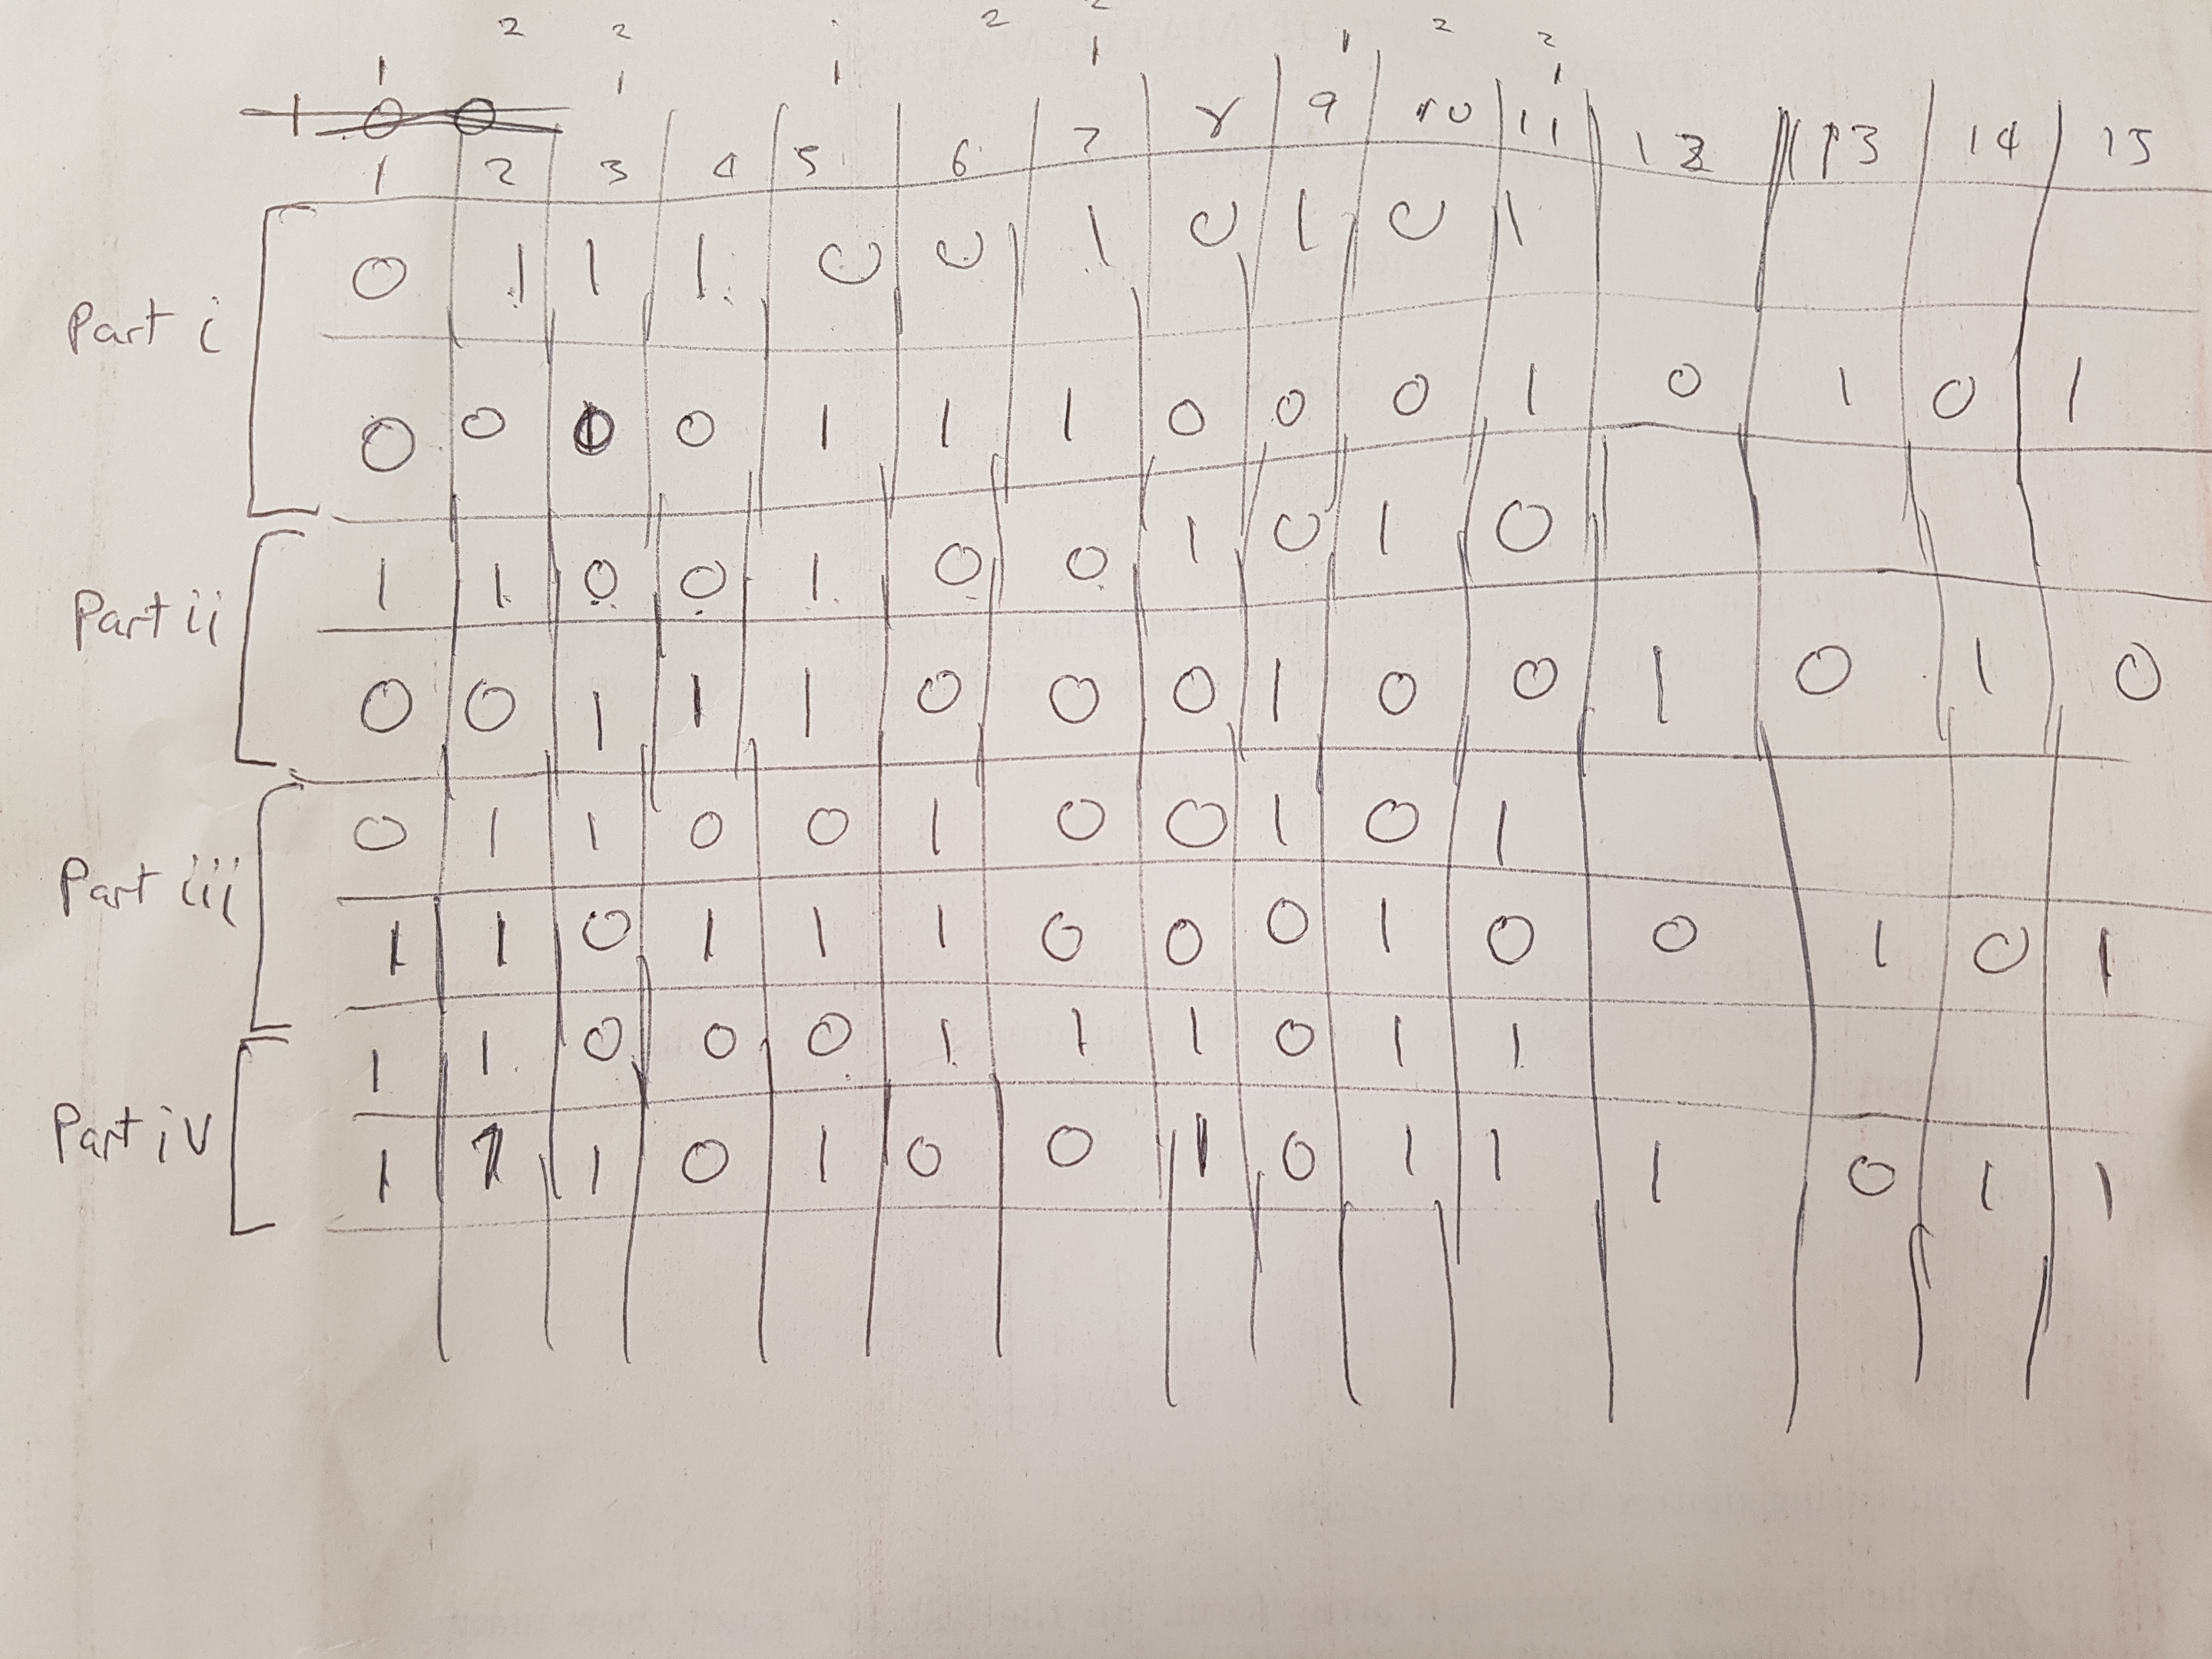
\includegraphics[width=5in]{working.jpg}
\end{figure}

\subsubsection{Part i}
$000011100010101$

\subsubsection{Part ii}
$001110001001010$

\subsubsection{Part iii}
$110111000100101$

\subsubsection{Part iv}
$111010010111011$

\subsection{Part c}
The following figure shows how I calculated the syndrome for each of the
received words.
\begin{figure}[H]
    \centering
    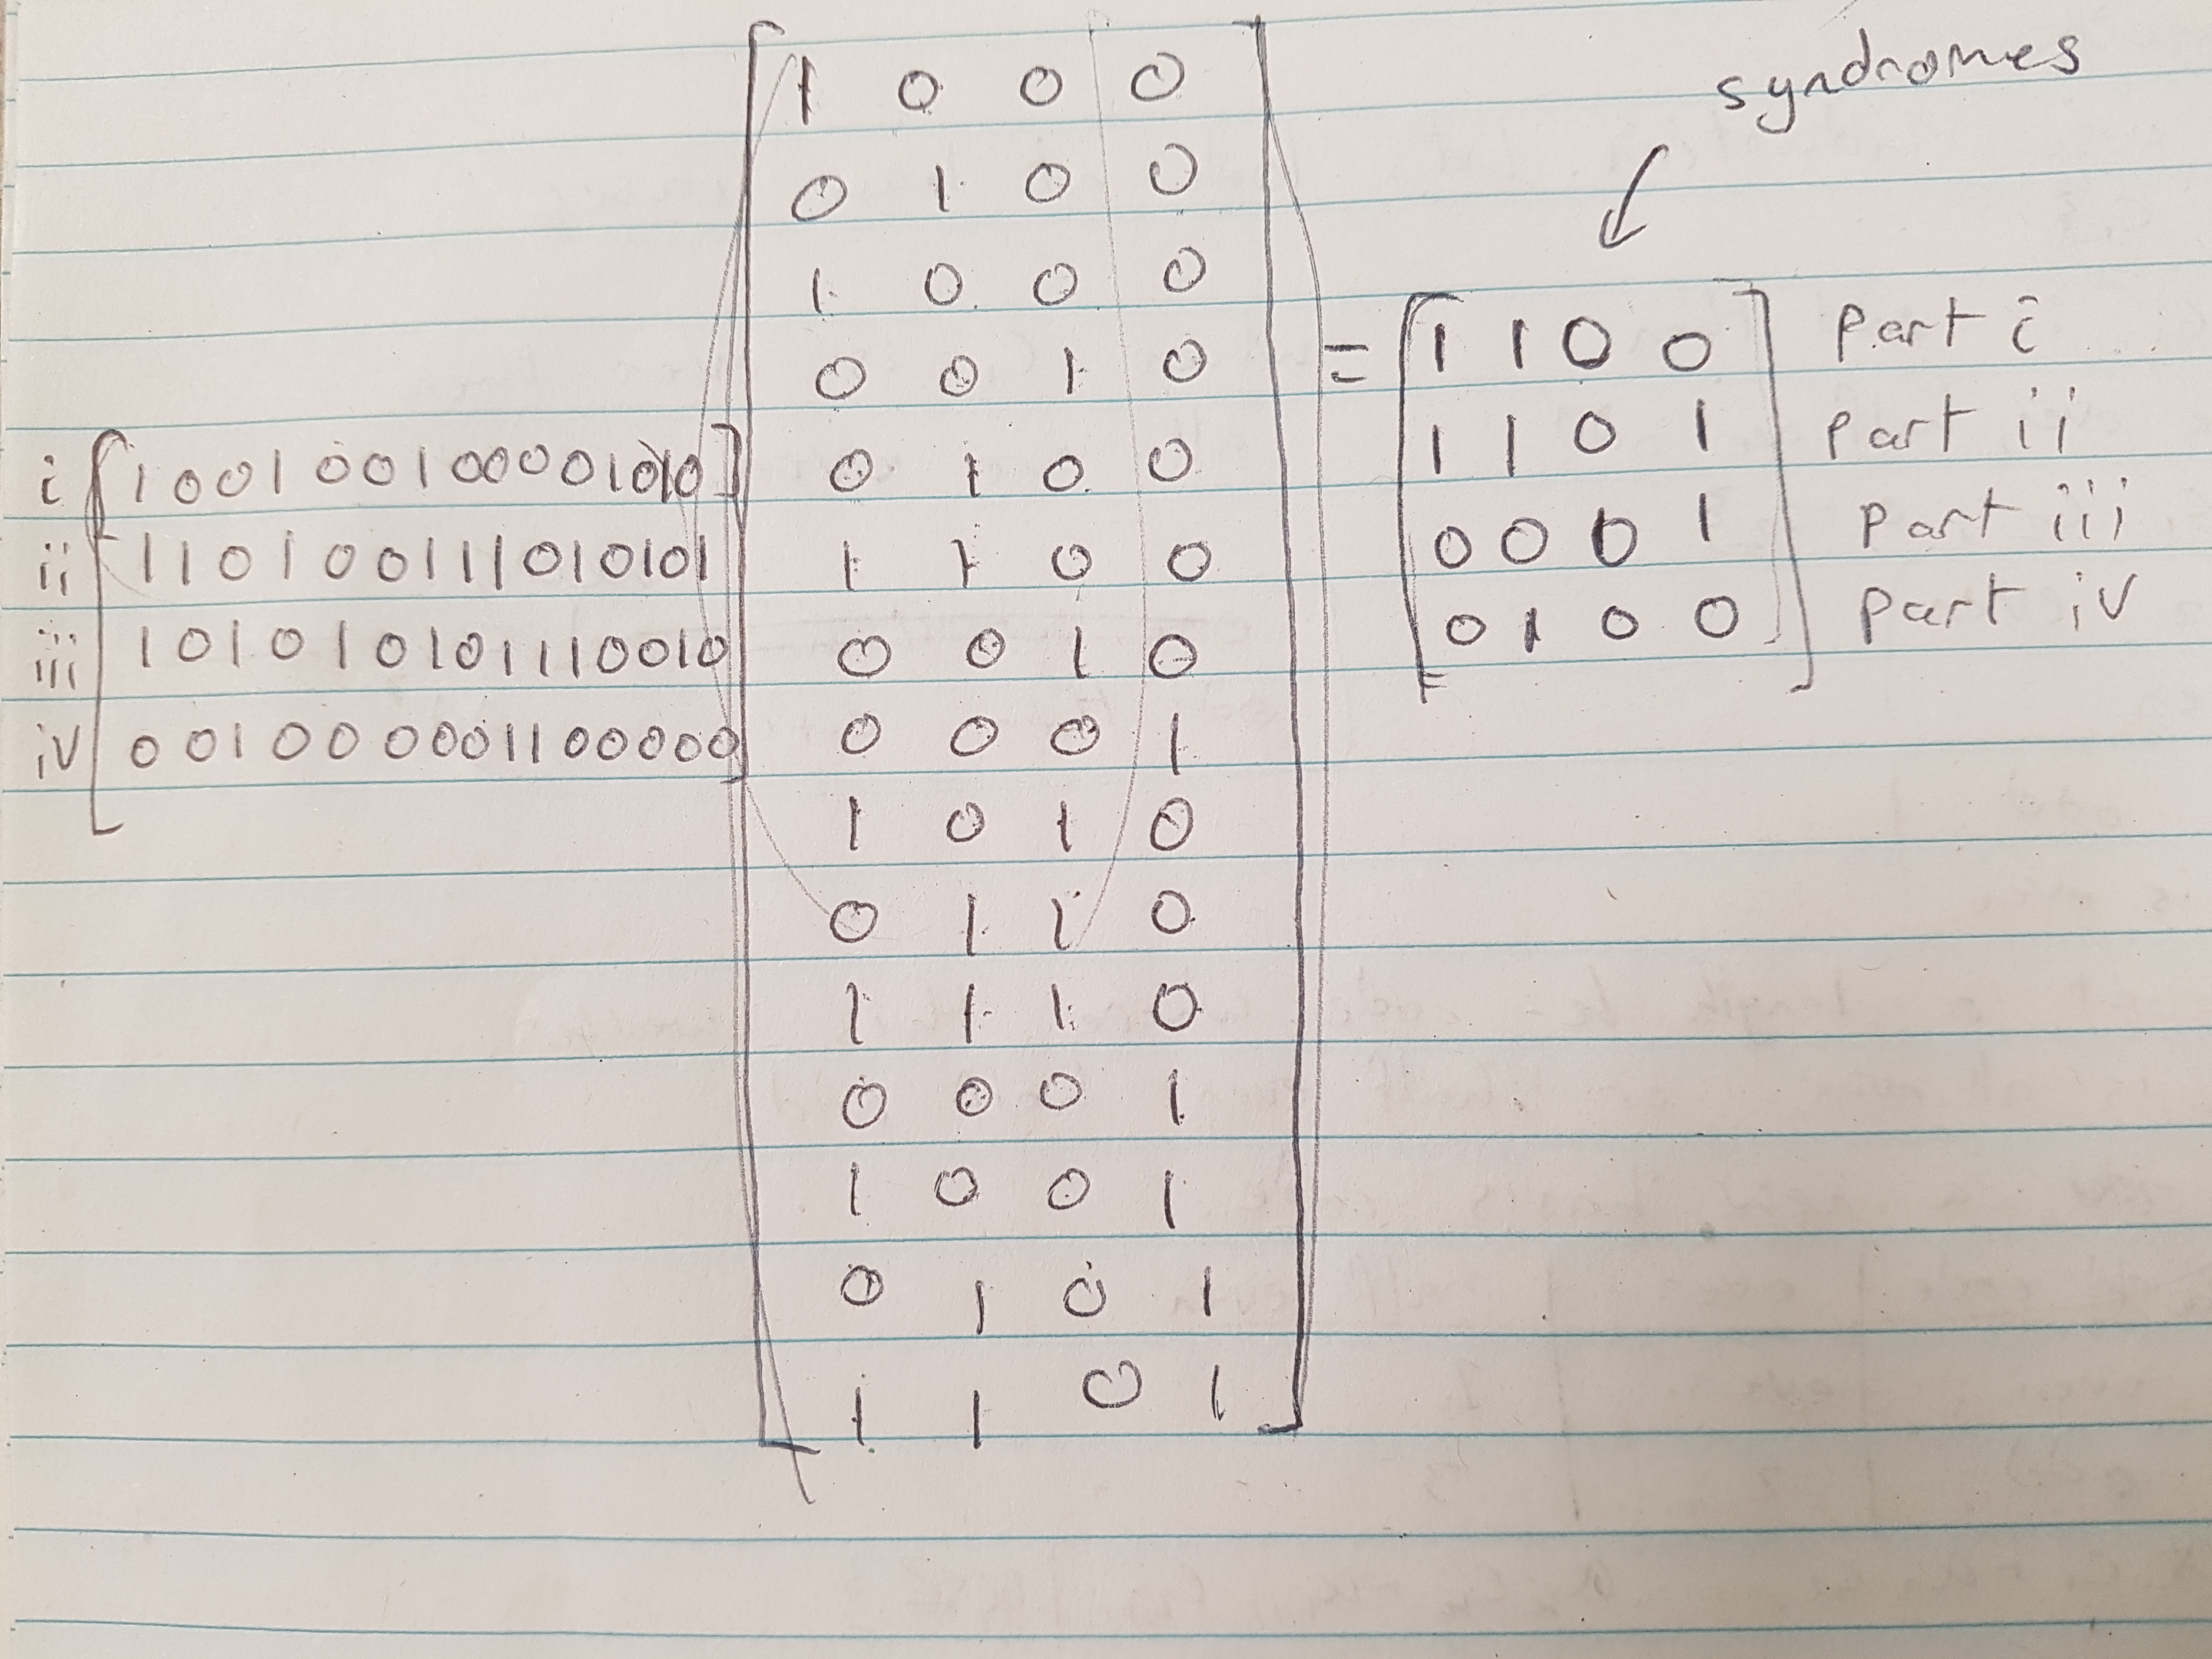
\includegraphics[width=5in]{syndrome.jpg}
\end{figure}

Since we know there is at most only one error in each of the words we only
have to determine the syndromes for an identity matrix, a single error in each
possible place. But because it's the identity matrix we will just have the
parity check matrix!

We now determine which bit was off by which row each syndrome equals.
\begin{enumerate}
    \item 6\textsuperscript{th} row
    \item 15\textsuperscript{th} row
    \item 12\textsuperscript{th} row
    \item 5\textsuperscript{th} row
\end{enumerate}

By subtracting a bit from the position corresponding to each word we should
get the original message. From there we can take the definition of the
Hamming code and decode each by taking all the bits that aren't a power of 2.

\subsubsection{Part i}
$100100100001010 \to 100101100001010 \to 00110001010$

\subsubsection{Part ii}
$110100111010101 \to 110100111010100 \to 00011010100$

\subsubsection{Part iii}
$101010101110010 \to 101010101111010 \to 11011111010$

\subsubsection{Part iv}
$001000001100000 \to 001010001100000 \to 11001100000$

\section{Problem Sheet 3 Question 6}
If all codes are $d=2t+1$ distance away from each other then the code is
capable of $t$ error correction, the nearest valid word is at most $t$ away.
So let's try and quantify the set all of all sequences that will correct to
a chosen word. Itself, Hamming distance 1, Hamming distance 2, etc.
For distance 0, there is only ${}^nC_0= 1$ possible option, the real code word.
For distance 1 there are ${}^nC_1$ possible error patterns, one for each
possible position of the single error. For distance 2, there are ${}^nC_2$
since any two position (ignoring order) can be chosen as the mutated bits.
This line of reasoning continues up to $t$ errors. Thus our final set of
correctable words is,
\begin{align*}
    |S| &= {}^nC_0 + {}^nC_1 + {}^nC_2 + {}^nC_3 + ... + {}^nC_t
\end{align*}

Since there are $|C|$ words in the code there should be $|C|$ of these $S$
sets. There will be no intersections of these sets since a word must be
uniquely corrected. But we also know the number of all possible words is
determined by the alphabet and the length of the words, $2^n$. Thus we
create our final statement,
\begin{align*}
    |C|\left({}^nC_0 + {}^nC_1 + {}^nC_2 + {}^nC_3 + ... + {}^nC_t\right)
    &\leq 2^n
\end{align*}

\section{Problem Sheet 3 Question 7}
Coding theory is essential in all activities in the modern, interconnected
world. One example of Coding Theory in the wild is actually in DDR RAM.
DDR uses an extension of Hamming codes to detect two errors, since the normal
Hamming code will only detect a single error (of which it will correct). This
modification of the classic encoding is called SECDED (Single Error Correction
Double Error Detection) in the industry. RAM is known to use this error
detection algorithm due to the low error rates present within a computer.
DDR RAM needs to be fast so data transfer needs to be high, Hamming code has
a rate of $1 - \frac{r}{2^r - 1}$ gets better and better rates at higher
lengths, (length being $2^r - 1$). The 
In comparison, deep space satellites like Voyager 1 and Voyager 2 use
Golay(24, 12, 8). Each word has distance 8 from each other giving a far
stronger encoding. The tradeoff for such robust codes is the low information
rate, $0.5$. If error detection and correction was not implemented in our
real world data communication we would find ourselves constantly dealing with
corrupted data. Data over large distance and large amount of information
would become impossible to send over the channels we take for granted today.

\end{document}
